\section{Mod\'elisation UML}

	\subsection{Cas d'utilisations}

\begin{figure}[H]
	\centering
	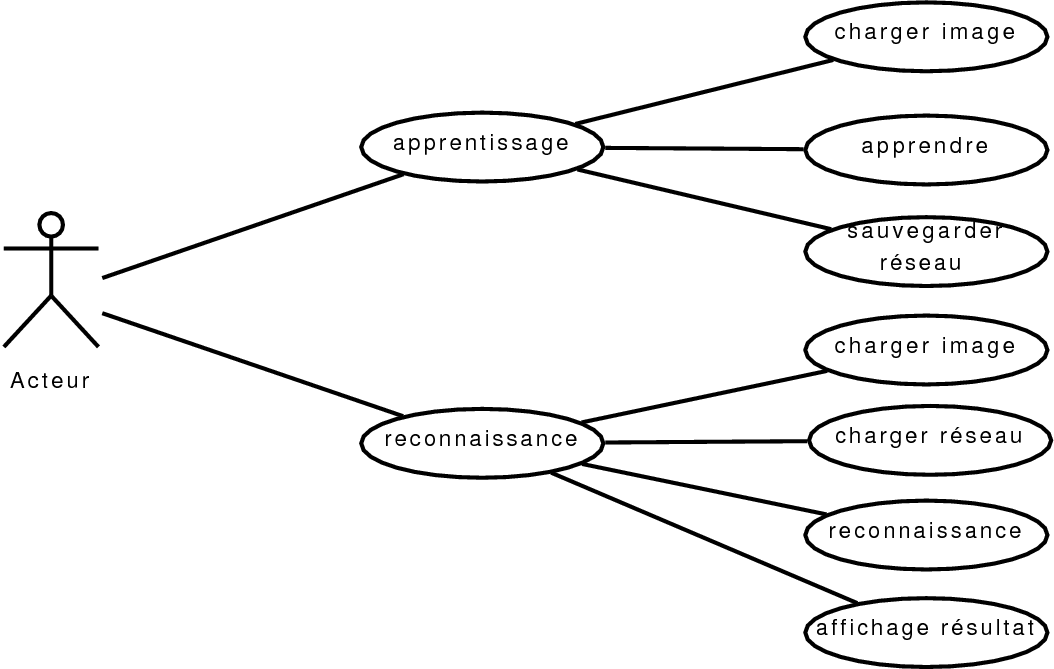
\includegraphics[width=0.8\linewidth]{diag/cas_utilisations.png}
\end{figure}

	\subsection{Modules}

\begin{figure}[H]
	\centering
	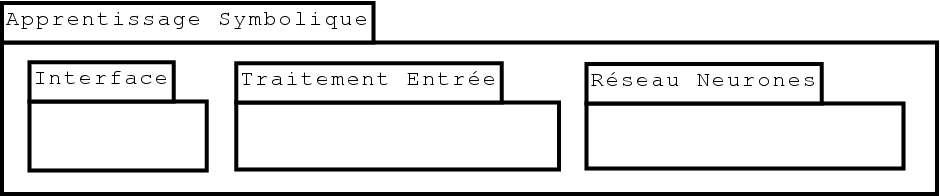
\includegraphics[width=0.8\linewidth]{diag/diag_package.png}
\end{figure}

	\subsubsection{Module Traitement Entr\'ees}

\begin{figure}[H]
	\centering
	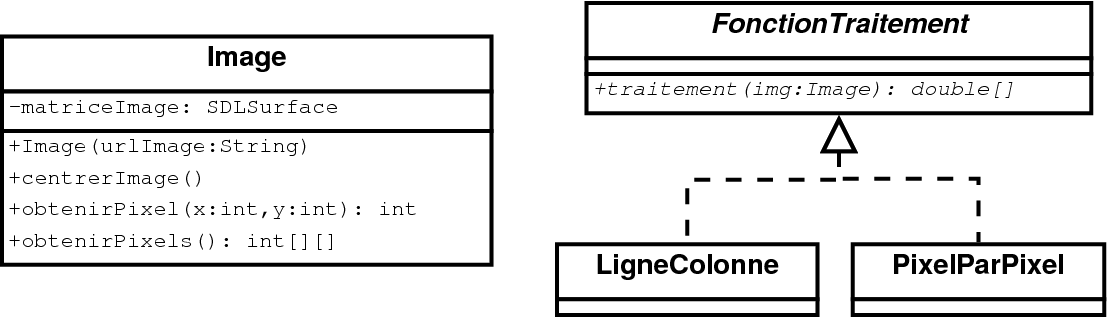
\includegraphics[width=0.7\linewidth]{diag/class_image.png}
\end{figure}

	\subsubsection{Module R\'eseau Neurones}
	
\begin{figure}[H]
	\centering
	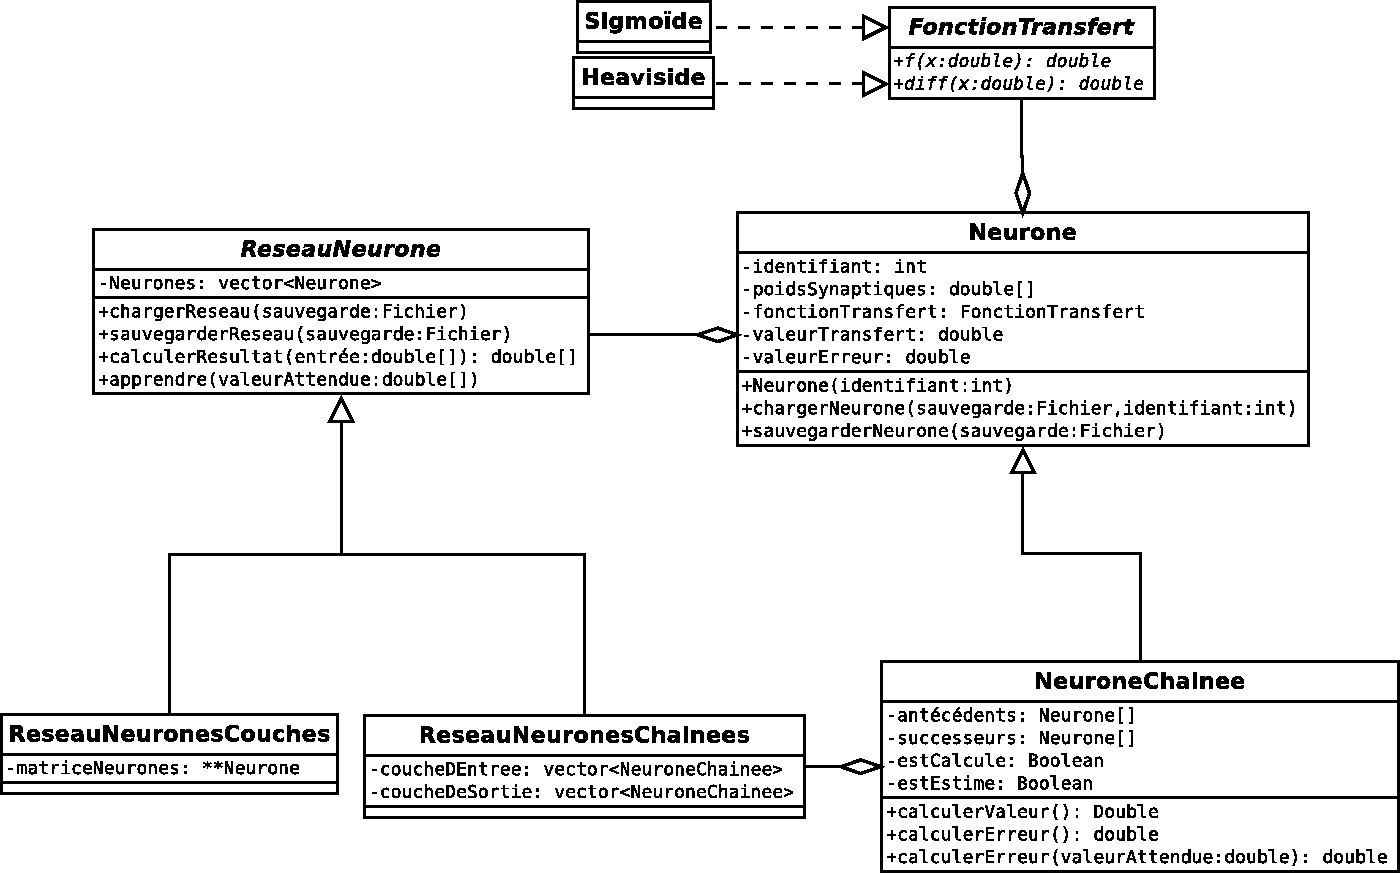
\includegraphics[width=1\linewidth]{diag/class_neurone.png}
\end{figure}

	\subsubsection{Module Interface}
	
\begin{figure}[H]
	\centering
	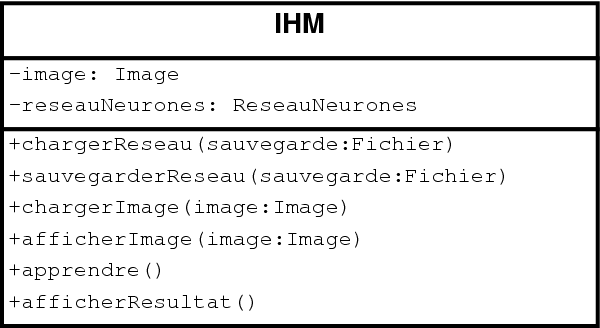
\includegraphics[width=0.4\linewidth]{diag/class_vue.png}
\end{figure}

	\subsection{Diagramme de séquence}

		\subsubsection{Apprentissage}
\begin{figure}[H]                                                                                                    
        \centering                                                                                                   
        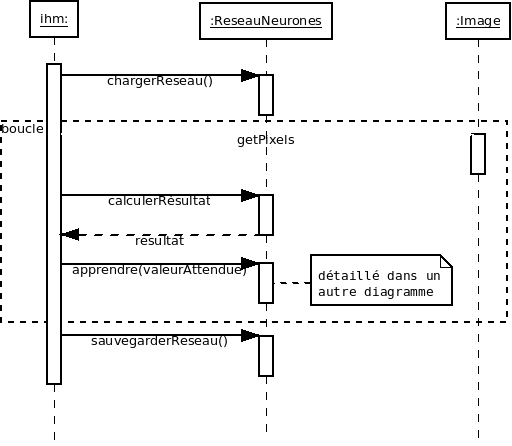
\includegraphics[width=0.6\linewidth]{diag/seq_apprentissage.png}                                                  
\end{figure}

		\subsubsection{Reconnaissance}
\begin{figure}[H]                                                                                                    
        \centering                                                                                                   
        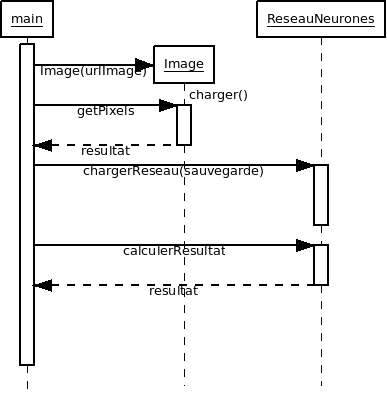
\includegraphics[width=0.6\linewidth]{diag/seq_reconnaissance.png}                                                  
\end{figure}

		\subsubsection{A continuer}